\documentclass[10pt]{article}
\usepackage[ngerman]{babel}
\usepackage[utf8]{inputenc}
\usepackage[T1]{fontenc}
\usepackage{amsmath}
\usepackage{amsfonts}
\usepackage{amssymb}
\usepackage[version=4]{mhchem}
\usepackage{stmaryrd}
\usepackage{graphicx}
\usepackage[export]{adjustbox}
\graphicspath{ {./images/} }

\title{Hauptprüfung Abiturprüfung 2023 - Leistungsfach }

\author{Alexander Schwarz\\
www.mathe-aufgaben.com}
\date{}


\begin{document}
\maketitle
 Baden-Württemberg

\section*{Aufgabe B2}
Die Abbildung in der Anlage zeigt den Körper ABCDEF mit $\mathrm{A}(6|3| 0), \mathrm{B}(0|6| 0)$, $\mathrm{C}(3|0| 0), \mathrm{D}(6|3| 6), \mathrm{E}(0|6| 6)$ und $\mathrm{F}(3|0| 12)$.\\
a) Die Punkte D, E und F liegen in der Ebene L.

Ermitteln Sie eine Gleichung von $L$ in Koordinatenform.\\
(Teilergebnis: $L: 2 x_{1}+4 x_{2}+3 x_{3}=42$ )\\
b) Bestimmen Sie die Größe des Winkels, den L mit der $\mathrm{x}_{1} \mathrm{x}_{2}$-Ebene einschließt.\\
(1,5 VP)\\
c) Der Flächeninhalt des Dreiecks ABC kann mit dem Term $6 \cdot 6-\frac{1}{2} \cdot 3 \cdot 3-2 \cdot \frac{1}{2} \cdot 3 \cdot 6$ berechnet werden. Veranschaulichen Sie diese Tatsache durch geeignete Eintragungen in der Abbildung.\\
(1,5 VP)\\
Berechnen Sie das Volumen des Körpers ABCDEF.\\
(1,5 VP)\\
d) Die Ebene $N_{k}$ enthält die $x_{3}$-Achse und den Punkt $P_{k}(1-k|k| 0)$ mit $\left.k \in\right] 0 ; 1[$. Welche Kanten des Körpers von $\mathrm{N}_{\mathrm{k}}$ geschnitten werden, ist abhängig von k . Durchläuft $k$ alle Werte zwischen 0 und 1 , so gibt es Bereiche ]a;b[, für die $N_{k}$ für alle Werte von $k \in] a ; b[$ jeweils die gleichen Kanten des Körpers schneidet. Bestimmen Sie den größten dieser Bereiche und geben Sie die zugehörigen Kanten an.\\
(2 VP)\\
e) Auf der Kante AD liegt der Punkt Q, auf der Kante BE der Punkt R(0|6|2).

Das Dreieck FQR hat in Q einen rechten Winkel.\\
Bestimmen Sie die $x_{3}$-Koordinate von $Q$.\\
f) Der Körper wird so um die Gerade $A B$ gedreht, dass der mit $D$ bezeichnete Eckpunkt nach der Drehung in der $\mathrm{x}_{1} \mathrm{x}_{2}$-Ebene liegt und dabei eine positive $\mathrm{x}_{2}$-Koordinate hat. Die folgenden Rechnungen liefern die Lösung einer Aufgabe im Zusammenhang mit der beschriebenen Drehung:

$$
\begin{aligned}
& \left(\begin{array}{c}
6 \\
-3 \\
0
\end{array}\right) \cdot\left[\left(\begin{array}{l}
0 \\
6 \\
0
\end{array}\right)+t \cdot\left(\begin{array}{c}
6 \\
-3 \\
0
\end{array}\right)-\left(\begin{array}{l}
3 \\
0 \\
0
\end{array}\right)\right]=0 \Leftrightarrow t=0,8 \text {, d.h. } S(4,8|3,6| 0) \\
& \overrightarrow{\mathrm{OT}}=\overrightarrow{\mathrm{OS}}+|\overrightarrow{\mathrm{CS}}| \cdot\left(\begin{array}{l}
0 \\
0 \\
1
\end{array}\right)
\end{aligned}
$$

Formulieren Sie eine passende Aufgabenstellung und geben Sie die Bedeutung von S an.

\section*{Anlage zu Aufgabe B2:}
\begin{center}
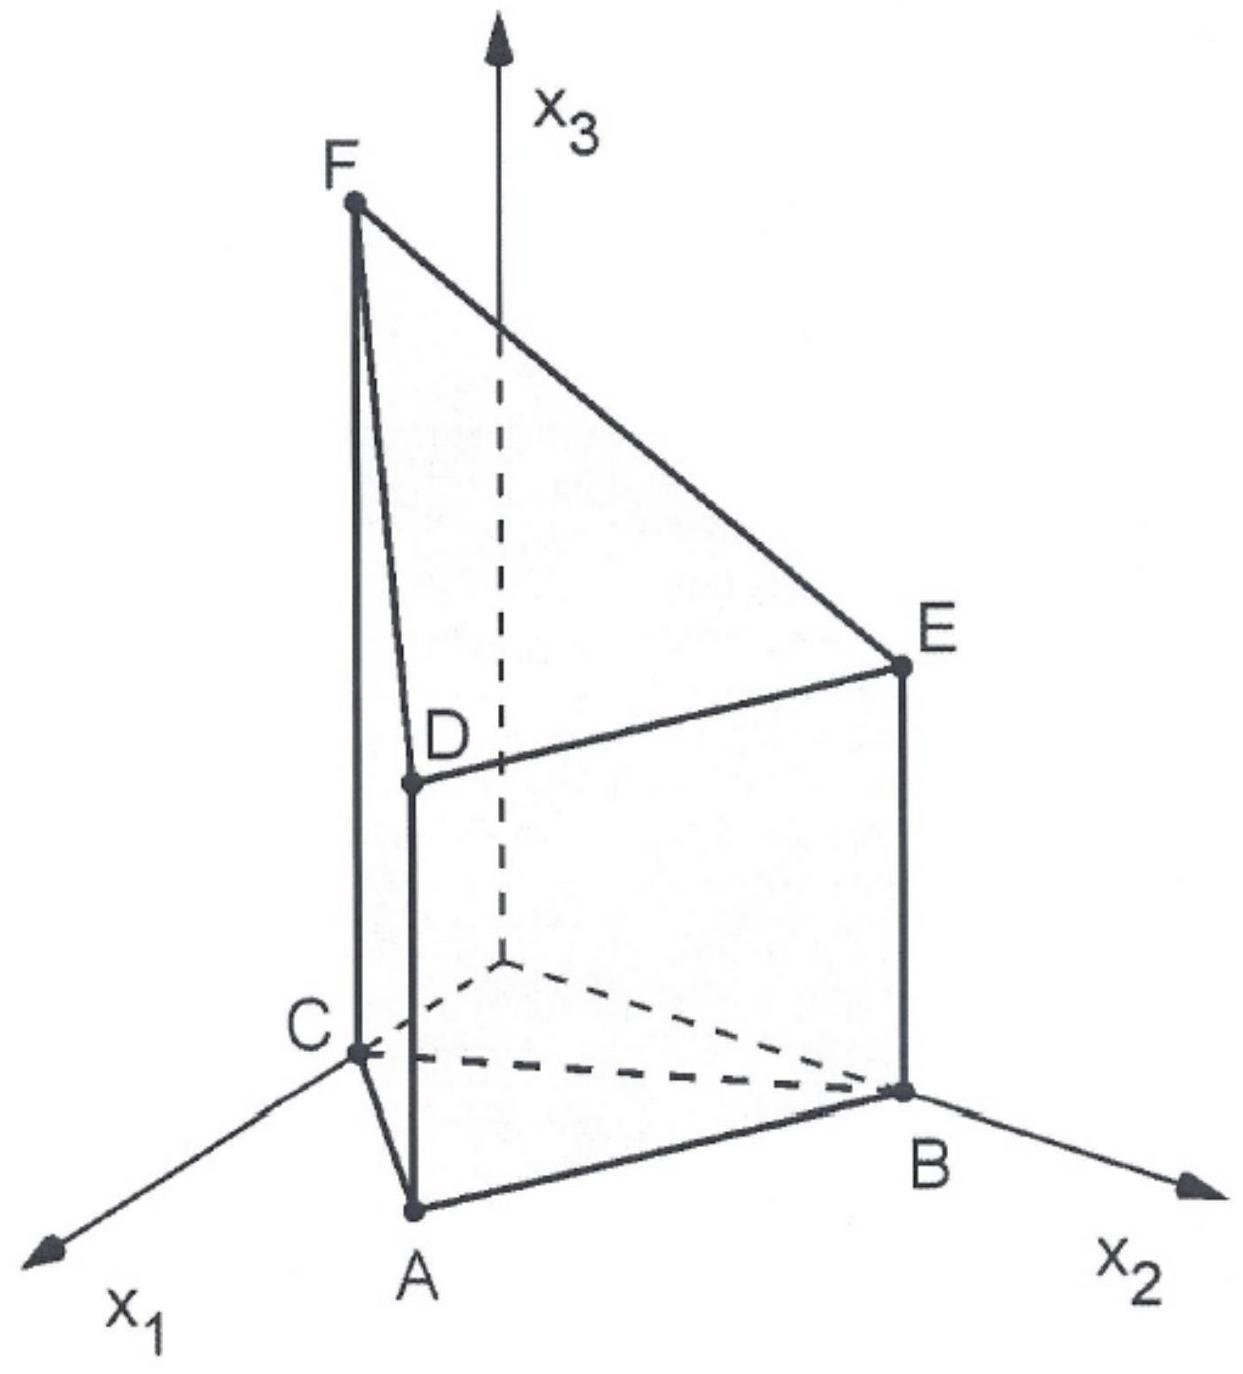
\includegraphics[max width=\textwidth]{2025_04_24_d093892bb0f2c23729d9g-3}
\end{center}

\section*{Lösungen}
\section*{Aufgabe B2}
a) Ermitteln Sie eine Gleichung von L in Koordinatenform.

Parameterform von $L: \vec{x}=\left(\begin{array}{l}6 \\ 3 \\ 6\end{array}\right)+r \cdot\left(\begin{array}{c}-6 \\ 3 \\ 0\end{array}\right)+s \cdot\left(\begin{array}{c}-3 \\ -3 \\ 6\end{array}\right)$\\
Normalenvektor von $\mathrm{L}: \overrightarrow{\mathrm{n}}=\left(\begin{array}{c}-6 \\ 3 \\ 0\end{array}\right) \times\left(\begin{array}{c}-3 \\ -3 \\ 6\end{array}\right)=\left(\begin{array}{l}18 \\ 36 \\ 27\end{array}\right)$ bzw. vereinfacht $\overrightarrow{\mathrm{n}}^{*}=\left(\begin{array}{l}2 \\ 4 \\ 3\end{array}\right)$\\
Ansatz der Koordinatenform: $\mathrm{L}: 2 \mathrm{x}_{1}+4 \mathrm{x}_{2}+3 \mathrm{x}_{3}=\mathrm{d}$\\
Einsetzen von $D(6|3| 6): 12+12+18=42 \Rightarrow d=42$\\
Koordinatenform: $L: 2 x_{1}+4 x_{2}+3 x_{3}=42$\\
b) Bestimmen Sie die Größe des Winkels, den L mit der $\mathrm{x}_{1} \mathrm{x}_{2}$-Ebene einschließt.

Die $x_{1} x_{2}$-Ebene besitzt den Normalenvektor $\vec{n}=\left(\begin{array}{l}0 \\ 0 \\ 1\end{array}\right)$\\
$\cos \alpha=\frac{\left(\left.\left(\begin{array}{l}2 \\ 4 \\ 3\end{array}\right) \cdot\left(\begin{array}{l}0 \\ 0 \\ 1\end{array}\right) \right\rvert\,\right.}{\sqrt{4+16+9 \cdot \sqrt{1}}}=\frac{3}{\sqrt{29}} \quad \Rightarrow \alpha \approx 56,1^{\circ}$\\
c) Veranschaulichen Sie diese Tatsache durch geeignete Eintragungen in der Abbildung.\\

Idee der Formel: $A_{\text {ABC }}=A_{\text {Quadrat }}-2 \cdot A_{\text {Dreieck OBC }}-A_{\text {Dreieck }}$

Berechnen Sie das Volumen des Körpers ABCDEF.\\
Der Körper setzt sich zusammen aus einem Prisma der Höhe 6 mit der Grundfläche ABC und einer darauf aufgesetzten Pyramide, deren Grundfläche genauso groß ist wie das Dreieck ABC (nur um 6 Längeneinheiten nach oben versetzt)\\
$A_{A B C}=6 \cdot 6-\frac{1}{2} \cdot 3 \cdot 3-2 \cdot \frac{1}{2} \cdot 3 \cdot 6=\frac{27}{2}$\\
$\mathrm{V}=\mathrm{V}_{\text {Prisma }}+\mathrm{V}_{\text {Pyramide }}=\mathrm{A}_{\mathrm{ABC}} \cdot \mathrm{h}_{\text {Prisma }}+\frac{1}{3} \cdot \mathrm{~A}_{\text {ABC }} \cdot \mathrm{h}_{\text {Pyramide }}=\frac{27}{2} \cdot 6+\frac{1}{3} \cdot \frac{27}{2} \cdot 6=108$\\
d) Bestimmen Sie den größten dieser Bereiche und geben Sie die zugehörigen Kanten an.

Die Ebene $N_{k}$ enthält die $x_{3}$-Achse und den Punkt $P_{k}(1-k|k| 0)$ mit $\left.k \in\right] 0 ; 1[$. Für k=0 (obwohl der Wert selbst nicht zulässig ist) ergäbe sich der Punkt $P_{0}(1|0| 0)$. Die Ebene $N_{0}$ wäre die $x_{1} x_{3}$-Ebene.\\
Für k = 1 (obwohl der Wert selbst nicht zulässig ist) ergäbe sich der Punkt $P_{1}(0|1| 0)$. Die Ebene $N_{1}$ wäre die $x_{2} x_{3}$-Ebene.\\
Somit stellt die Ebenenschar $\mathrm{N}_{\mathrm{k}}$ alle Ebenen dar, die sich zwischen der $\mathrm{x}_{1} \mathrm{x}_{3}$-Ebene und der $\mathrm{x}_{2} \mathrm{x}_{3}$-Ebene bewegen und die $\mathrm{x}_{3}$-Achse enthalten.

Bewegt sich die Ebenenschar von der $\mathrm{x}_{1} \mathrm{x}_{3}$-Ebene entgegen dem Uhrzeigersinn weg, schneiden sich die Ebenen in den Kanten AC, FD, FE und BC.\\
Dies gilt so lange, bis die Ebenenschar die Gerade durch OA enthält.\\
Gleichung der Geraden OA: $g: \vec{x}=\left(\begin{array}{l}0 \\ 0 \\ 0\end{array}\right)+r \cdot\left(\begin{array}{l}6 \\ 3 \\ 0\end{array}\right)$\\
Prüfung, für welchen Wert von $k$ die Punkteschar $P_{k}$ auf $g$ liegt:\\
$\left(\begin{array}{c}1-k \\ k \\ 0\end{array}\right)=\left(\begin{array}{l}0 \\ 0 \\ 0\end{array}\right)+r \cdot\left(\begin{array}{l}6 \\ 3 \\ 0\end{array}\right) \Rightarrow \begin{array}{cc}1-k & =6 r \\ k & =3 r\end{array}$\\
Einsetzen von der 2.Zeile in die 1.Zeile: $1-3 r=6 r \Rightarrow r=\frac{1}{9}$\\
Daraus folgt $\mathrm{k}=\frac{1}{3}$.\\
Für $k \in] 0 ; \frac{1}{3}[$ schneiden sich die Ebenen in den Kanten AC, FD, FE und BC.

Für $k \in] \frac{1}{3} ; 1[$ schneiden sich die Ebenen in den Kanten $A B, D E$, FE und $B C$.\\
Dies ist der gesuchte größte Bereich.\\
e) Bestimmen Sie die $\mathrm{x}_{3}$-Koordinate von Q .

Der Punkt $Q$ hat die Koordinaten $Q(6|3| \mathrm{u})$ mit $0 \leq \mathrm{u} \leq 6$.\\
Da im Punkt Q sich ein rechter Winkel befindet muss gelten:\\
$\overrightarrow{\mathrm{QF}} \cdot \overrightarrow{\mathrm{QR}}=0 \Leftrightarrow\left(\begin{array}{c}-3 \\ -3 \\ 12-\mathrm{u}\end{array}\right) \cdot\left(\begin{array}{c}-6 \\ 3 \\ 2-\mathrm{u}\end{array}\right)=0 \Leftrightarrow 18-9+24-14 \mathrm{u}+\mathrm{u}^{2}=0$\\
$\Leftrightarrow u^{2}-14 u+33=0 \quad \Rightarrow u_{1,2}=\frac{14 \pm \sqrt{196-132}}{2}=\frac{14 \pm 8}{2} \quad u_{1}=11 \quad u_{2}=3$\\
Da $0 \leq \mathrm{u} \leq 6$ gelten muss, ist die $\mathrm{x}_{3}$-Koordinate von Q gleich 3 .\\
f) Formulieren Sie eine passende Aufgabenstellung und geben Sie die Bedeutung von S an.

Der Term $\left(\begin{array}{l}0 \\ 6 \\ 0\end{array}\right)+\mathrm{t} \cdot\left(\begin{array}{c}6 \\ -3 \\ 0\end{array}\right)$ gibt die\\
Parameterform der Geraden g an, die durch $A$ und $B$ verläuft.\\
Wenn $t=0,8$ in die Geradengleichung $g$ eingesetzt wird, ergibt sich der Punkt S.\\
Somit muss $S$ auf g liegen.\\
Aus der Formel $\overrightarrow{\mathrm{OT}}=\overrightarrow{\mathrm{OS}}+|\overrightarrow{\mathrm{CS}}| \cdot\left(\begin{array}{l}0 \\ 0 \\ 1\end{array}\right)$\\
kann man ablesen:\\
Der Punkt T befindet sich genau oberhalb vom Punkt $S$ mit dem Abstand $\overline{\mathrm{CS}}$.

Der Term $\left(\begin{array}{l}0 \\ 6 \\ 0\end{array}\right)+t \cdot\left(\begin{array}{c}6 \\ -3 \\ 0\end{array}\right)-\left(\begin{array}{l}3 \\ 0 \\ 0\end{array}\right)$ beschreibt den Vektor $\overrightarrow{\mathrm{CS}}$, der vom Punkt $\mathrm{C}(3|0| 0)$ auf einen Punkt $S$ der Gerade g zeigt.

Da das Skalarprodukt $\left(\begin{array}{c}6 \\ -3 \\ 0\end{array}\right) \cdot\left[\left(\begin{array}{l}0 \\ 6 \\ 0\end{array}\right)+\mathrm{t} \cdot\left(\begin{array}{c}6 \\ -3 \\ 0\end{array}\right)-\left(\begin{array}{l}3 \\ 0 \\ 0\end{array}\right)\right]=0$ ist, muss der Vektor $\overrightarrow{\mathrm{CS}}$ senkrecht auf der Geraden g stehen.

Da der Körper um die Gerade AB um $90^{\circ}$ gedreht wird, entspricht der Punkt T dem Punkt $C^{\prime}$, der aus dem Punkt $C$ nach der Drehung des Körpers übergeht.

Bedeutung von S:\\
$S$ ist der Fußpunkt des Lots von C auf die Gerade AB.\\
Aufgabenstellung:\\
Der mit C bezeichnete Eckpunkt des Körpers wird nach der Drehung mit T bezeichnet. Ermitteln Sie die Koordinaten von T.


\end{document}